\subsection{Support Vector Machine (SVM)}
\label{sec:SVM}

In the early 1960s a linear support vector method\index{Support vector machine, SVM}
has been developed for the construction of
separating hyperplanes for pattern recognition problems~\cite{Vapnik1963,Vapnik1964}. 
It took 30 years before the method was generalised to nonlinear separating 
functions~\cite{Vapnik1992,Vapnik1995a} and for estimating real-valued functions 
(regression)~\cite{Vapnik1995b}. At that moment it became a general purpose algorithm, 
performing classification and regression tasks which can compete with neural networks 
and probability density estimators. Typical applications of SVMs include text 
categorisation, character recognition, bio-informatics and face detection. 

The main idea of the SVM approach to classification problems is to build a hyperplane 
that separates signal and background {\em vectors} (events) using only a minimal subset 
of all training vectors ({\em support vectors}). The position of the hyperplane is 
obtained by maximizing the margin (distance) between it and the support vectors.  
The extension to nonlinear SVMs is performed by mapping the input vectors onto 
a higher dimensional feature space in which signal and background events can be 
separated by a linear procedure using an optimally separating hyperplane. The use 
of kernel functions eliminates thereby the explicit transformation to the feature 
space and simplifies the computation.

The implementation of the newly introduced regression is similar to the approach in classification.
It also maps input data into higher dimensional space using previously chosen support 
vectors. Instead of separating events of two types, it determines the hyperplane with 
events of the same value (which is equal to the {\em mean} from all training events). 
The final value is estimated based on the distance to the hyperplane which is computed by the selected kernel function.% Comment: currently we can only select Gaus, soon we will have most of the old kernel options back
\subsubsection{Booking options}

The SVM classifier is booked via the command:
\begin{codeexample}
\begin{tmvacode}
factory->BookMethod( TMVA::Types::kSVM, "SVM", "<options>" ); 
\end{tmvacode}
\caption[.]{\codeexampleCaptionSize Booking of the SVM classifier: the first  
            argument is a unique type enumerator, the second is a user-defined  
            name which must be unique among all booked classifiers, and the third argument 
            is the configuration option string. Individual options are separated by a ':'. 
            For options that are not set in the string default values are used. 
            See Sec.~\ref{sec:usingtmva:booking} for more information on the booking.}
\end{codeexample}

The configuration options for the SVM classifier are given in Option Table~\ref{opt:mva::svm}.


% ======= input option table ==========================================
\begin{option}[t]
\input optiontables/MVA__SVM.tex
\caption[.]{\optionCaptionSize 
     Configuration options reference for MVA method: {\em SVM}.
     Values given are defaults. If predefined categories exist, the default category 
     is marked by a '$\star$'. The options in Option Table~\ref{opt:mva::methodbase} on 
     page~\pageref{opt:mva::methodbase} can also be configured.     
%     Definition of the kernel function: \code{Linear} is 
%     $K(\vec x, \vec y) = \vec x \cdot \vec y $ (no extra parameters),
%     \code{Polynomial} is $K(\vec x, \vec y) = (\vec x \cdot \vec y +\theta)^d$,
%     \code{Gauss} is 
%     $K(\vec x, \vec y) = \exp\big(-\left|\vec x - \vec y \right|^2 /2\sigma^2\big)$,
%     and \code{Sigmoid} corresponds to
%     $K(\vec x, \vec y) = \tanh\left(\kappa (\vec x \cdot \vec y) +\theta \right)$
}
\label{opt:mva::svm}
\end{option}
% =====================================================================

\subsubsection{Description and implementation}

A detailed  description of the SVM formalism can be found, for example,
in Ref.~\cite{Burges}. Here only a brief introduction of the TMVA 
implementation is given. 

\subsubsection*{Linear SVM}
\index{Support vector machine, SVM!linear}

%
\begin{figure}[t]
\centering
	  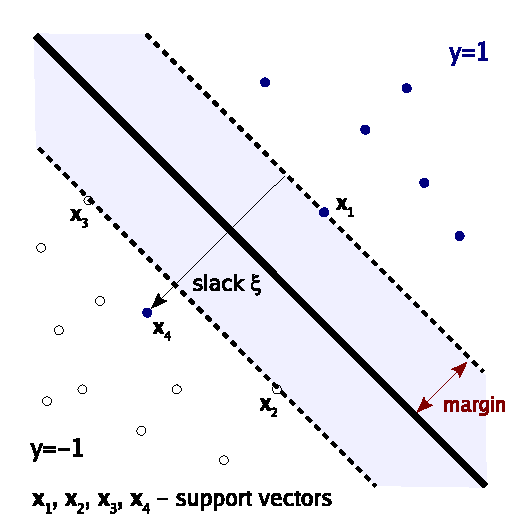
\includegraphics[width=0.47\textwidth]{plots/SVM}
\caption{ Hyperplane classifier in two dimensions. The vectors (events) ${\bf x}_{1-4}$          
          define the hyperplane and margin, \ie, they are the support vectors.
}
\label{fig:classifier}
\end{figure}
Consider a simple two-class classifier  with oriented hyperplanes.  If the training 
data is linearly separable, a vector-scalar pair $(\vec w, b)$ can be found that 
satisfies the constraints
%
\beq
   \label{eq:SVM1}
   y_i (\vec {x_i}\cdot \vec w+ b)-1 \ge 0\,, \space \mbox{\hspace{0.5cm}} \forall_i\,,
\eeq
%
where $\vec x_i$ are the input vectors, $y_i$ the desired outputs ($y_i=\pm 1$),  
and where the pair $(\vec w,b)$ defines a hyperplane. The decision function of 
the classifier is  
$f(\vec x_i)= {\rm sign} (\vec x_i\cdot \vec w+ b)$, which is $+1$ for all points on   
one side of the hyperplane and $-1$ for the points on the other side. 

Intuitively, the classifier with the largest margin will give better separation.
The margin for this linear classifier is just $2/|\vec w|$.  Hence to maximise the 
margin, one needs to minimise the {\em cost function} $W = |\vec w|^2/w$ with the 
constraints from Eq.~(\ref{eq:SVM1}). 

At this point it is beneficial to consider the significance of different input  
vectors $\vec x_i$.  The training events lying on the margins, which are called  
the support vectors (SV), are the events that contribute to defining the decision boundary  
(see Fig.~\ref{fig:classifier}). Hence if the other events are removed from the training 
sample and the classifier is retrained on the remaining events, the training will result 
in the same decision boundary. To solve the constrained quadratic optimisation problem, 
we first reformulate it in terms of a Lagrangian
%
\beq
   {\cal L}( \vec w, b, \vec \alpha) = \frac{1}{2}\left| \vec w \right|^2-
   \sum_i \alpha_i \left( y_i \left( ( \vec x_i \cdot \vec w ) + b\right)-1\right)
\eeq
%
where $\alpha_i \ge 0$ and the condition from Eq.~(\ref{eq:SVM1}) must be fulfilled. 
The Lagrangian ${\cal L}$ is minimised with respect to $\vec w$ and $b$  and  
maximised  with respect to $\vec \alpha$. The solution has an expansion in terms  
of a subset of input vectors for which $\alpha_i \ne 0$ (the support vectors):
%
\beq
   \vec w = \sum_i \alpha_i y_i \vec x_i\,,
\eeq
%
because $\partial {\cal L} / \partial b =0$ and $\partial {\cal L}/\partial\vec w=0$
hold at the extremum. The optimisation problem translates to finding the vector 
$\vec \alpha$ which maximises
%
\beq
\label{eq:SVMdot}
   {\cal L}( \vec \alpha )=  \sum_i \alpha_i - 
   \frac{1}{2}  \sum_{ij} \alpha_i \alpha_j y_i y_j \vec x_i \cdot \vec x_j \,.
\eeq
%
Both the optimisation problem and the final decision function depend only on scalar  
products between input vectors, which is a crucial property for the generalisation 
to the nonlinear case.

\subsubsection*{Nonseparable data}
\label{SVM:nonseparable}
\index{Nonseparable data}

The above algorithm can be extended to non-separable data. The classification  
constraints in Eq.~(\ref{eq:SVM1}) are modified by adding a ``slack'' variable $\xi_i$ to  
it ($\xi_i=0$ if the vector is properly classified, otherwise $\xi_i$ is the distance  
to the decision hyperplane)
%
\beq
\label{eq:SVM2}
   y_i (\vec {x_i}\cdot \vec w+ b)-1 +\xi_i \ge 0,\space 
   \mbox{\hspace{1cm}} \xi_i\ge 0\,, \mbox{\hspace{0.5cm}} \forall_i\,.
\eeq
%
This admits a certain amount of misclassification. The training algorithm thus
minimises the modified cost function 
%
\beq
\label{eq:SVM3}
   W = \frac{1}{2}\left| \vec w \right|^2 + C \sum_i \xi_i\,,
\eeq
describing a trade-off between margin and misclassification. The cost parameter \code{C} 
sets the scale by how much misclassification increases the cost function (see Tab.~\ref{opt:mva::svm}).

\subsubsection*{Nonlinear SVM}
\index{Support vector machine, SVM!nonlinear}

The SVM formulation given above can be further extended to build a nonlinear  
SVM which can classify nonlinearly separable data.
%
Consider a function $\Phi:\;{\rm R}^\Nvar\to\cal H$, which maps the training data 
from ${\rm R}^\Nvar$, where $\Nvar$ is the number of discriminating input variables, 
to some higher dimensional space $\cal H$. In the $\cal H$ space the signal and background 
events can be linearly separated so that the linear SVM formulation can be applied. We have 
seen in Eq.~(\ref{eq:SVMdot}) that event variables only appear in the form of 
scalar products  $\vec x_i\cdot \vec x_j$, which become $\Phi(\vec x_i)\cdot \Phi(\vec x_j)$ 
in the higher dimensional feature space $\cal H$. The latter scalar product can be approximated 
by a kernel function
%
\beq
   K(\vec x_i, \vec x_j)\approx\Phi(\vec x_i)\cdot \Phi(\vec x_j)\,,
\eeq
%
which avoids the explicit computation of the mapping function $\Phi(\vec x)$. 
This is desirable because the exact form of $\Phi(\vec x)$ is hard to derive from
the training data. Most frequently used kernel functions are
%
\beq
\label{SMV:kernels}
\def\smallEq{\hspace{-0.15cm}=}
\begin{array}{rcll}
  K(\vec x, \vec y) &\smallEq
                      &\hspace{-0.15cm} (\vec x \cdot \vec y +\theta)^d 
                      &\hspace{0.2cm}\text{\em Polynomial}, \\ 
  K(\vec x, \vec y) &\smallEq
                      &\hspace{-0.15cm} \exp\left(-\left|\vec x - \vec y \right|^2 /2\sigma^2\right) 
                      &\hspace{0.2cm} \text{\em Gaussian}, \\
  K(\vec x, \vec y) &\smallEq
                     &\hspace{-0.15cm} \tanh\left(\kappa (\vec x \cdot \vec y) +\theta\right) 
                     &\hspace{0.2cm} \text{\em Sigmoidal},
\end{array}
\eeq
of which currently only the Gaussian Kernel is implemented in TMVA.
%
It was shown in Ref.~\cite{Vapnik1995b} that a suitable function kernel must fulfill  
Mercer's condition
%
\beq
   \int K(\vec x, \vec y)g(\vec x)g(\vec y)d\vec x d\vec y \ge 0\,,
\eeq
%
for any function $g$ such that $\int g^2(\vec x) d\vec x$ is finite.
While Gaussian and polynomial kernels are known to comply with Mercer's condition,  
this is not strictly the case for sigmoidal kernels. To extend the linear 
methodology to nonlinear problems one substitutes  $\vec x_i \cdot \vec x_j$ 
by $K(\vec x_i, \vec x_j)$ in Eq.~(\ref{eq:SVMdot}).
Due to Mercer's conditions on the kernel, the corresponding optimisation problem  
is a well defined convex quadratic programming problem with a global minimum. 
This is an advantage of SVMs compared to neural networks where local minima occur.

For regression problems, the same algorithm is used as for classification with the exception that instead of dividing 
events based on their type (signal/background), it separates them based on the value
(larger/smaller than average). In the end, it does not return the sigmoid of the distance 
between the event and the hyperplane, but the distance itself -- increased by the average target value. 

\subsubsection*{Implementation}

The TMVA implementation of the Support Vector Machine follows closely the description  
given in the literature. It employs a sequential minimal optimisation (SMO)~\cite{Platt}  
to solve the quadratic problem. Acceleration of the minimisation is achieved by dividing
a set of vectors into smaller subsets~\cite{Keerthi}. The number of training subsets is 
controlled by option \code{NSubSets}. The SMO method drives the subset 
selection to the extreme by selecting subsets of two vectors (for details see 
Ref.~\cite{Burges}). The pairs of vectors are chosen, using heuristic rules, to achieve
the largest possible improvement (minimisation) per step. Because the working set is of 
size two, it is straightforward to write down the analytical solution. The minimisation 
procedure is repeated recursively until the minimum is found. The SMO algorithm has proven 
to be significantly faster than other methods and has become the most common  
minimisation method used in SVM implementations. The precision of the minimisation 
is controlled by the tolerance parameter \code{Tol} (see Tab.~\ref{opt:mva::svm}). The 
SVM training time can be reduced by increasing the tolerance. Most classification problems 
should be solved with less then 1000 training iterations. Interrupting the SVM algorithm 
using the option \code{MaxIter} may thus be helpful when optimising the SVM training 
parameters.  \code{MaxIter} can be released for the final classifier training.

\subsubsection{Variable ranking}

The present implementation of the SVM classifier does not provide a ranking 
of the input variables.

\subsubsection{Performance}
\label{SVM:performance}
\index{Support vector machine, SVM!performance of}

%The TMVA SVM algorithm comes with linear, polynomial, Gaussian and sigmoidal kernel functions.
The TMVA SVM algorithm comes currently only with the Gaussian kernel function.
With sufficient training statistics, the Gaussian kernel allows to approximate 
any separating function in the input space. It is crucial for the performance of the
SVM to appropriately tune the kernel parameters and the cost parameter \code{C}. 
In case of a Gaussian, the kernel is tuned via option \code{Gamma} which is related to 
the width $\sigma$ by $\Gamma=1/(2 \sigma^2)$.
The optimal tuning of these parameters is specific to the problem and must be done by the user. 

The SVM training time scales with $n^2$, where $n$ is the number of vectors (events) in   
the training data set. The user is therefore advised to restrict the sample size
during the first rough scan of the kernel parameters. Also increasing the minimisation
tolerance helps to speed up the training.

SVM is a nonlinear general purpose classification and regression algorithm with 
a performance similar to neural networks (Sec.~\ref{sec:ann}) or to a multidimensional 
likelihood estimator (Sec.~\ref{sec:pders}).
